\documentclass{article}
\usepackage{tikz, comment}
\usepackage{pifont}
\usepackage{fontspec}
\usetikzlibrary{arrows, decorations.markings, decorations.pathreplacing}
\begin{comment}
:Title: Not defined yet
:Tags: moment;perimeter;difference quotient;apothem;directrix of a parabola
:Prob: 0.427;0.4121;0.4055;0.3963;0.3947
:Slug: No name yet

Description Here.........
\end{comment}
\begin{document}\centering

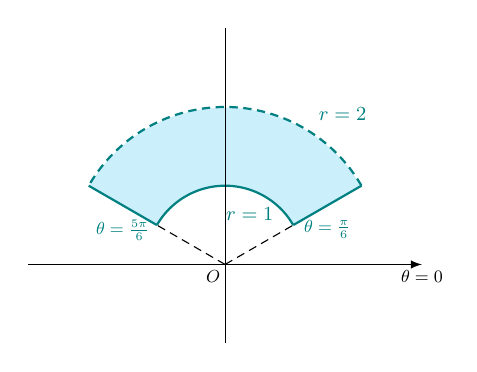
\begin{tikzpicture}[>=latex,xscale=.5*2, yscale=.5*2][font=\sf\small]

%\draw[xstep=1cm,ystep=1cm,color=gray!80] (0, -1) grid (8, 8);

\draw[white, fill=cyan!20, samples=100, smooth, domain=pi/6:5*pi/6, variable=\t]
plot ({2*cos(\t r)}, {2*sin(\t r)})--(0, 0);

\draw[white, fill=white, samples=100, smooth, domain=pi/6:5*pi/6, variable=\t]
plot ({1*cos(\t r)}, {1*sin(\t r)})--(0, 0);

\draw[teal, thick, densely dashed, samples=100, smooth, domain=pi/6:5*pi/6, variable=\t]
plot ({2*cos(\t r)}, {2*sin(\t r)});
\draw[teal, thick, samples=100, smooth, domain=pi/6:5*pi/6, variable=\t]
plot ({1*cos(\t r)}, {1*sin(\t r)});

\draw[teal, thick] ({1*cos(pi/6 r)}, {1*sin(pi/6 r)})--({2*cos(pi/6 r)}, {2*sin(pi/6 r)});
\draw[teal, thick] ({1*cos(5*pi/6 r)}, {1*sin(5*pi/6 r)})--({2*cos(5*pi/6 r)}, {2*sin(5*pi/6 r)});

\draw[densely dashed] ({0*cos(pi/6 r)}, {0*sin(pi/6 r)})--({1*cos(pi/6 r)}, {1*sin(pi/6 r)});
\draw[densely dashed] ({0*cos(5*pi/6 r)}, {0*sin(5*pi/6 r)})--({1*cos(5*pi/6 r)}, {1*sin(5*pi/6 r)});

\node[teal, left, yshift=-2, scale=0.8] at ({1*cos(pi/4 r)}, {1*sin(pi/4 r)}) {$r=1$};
\node[teal, right, scale=0.8] at ({2.2*cos(pi/3 r)}, {2.2*sin(pi/3 r)}) {$r=2$};

\node[teal, below, yshift=-3, scale=0.7] at ({1.5*cos(1*pi/6 r)}, {1.5*sin(1*pi/6 r)}) {$\theta=\frac{\pi}{6}$};
\node[teal, below, yshift=-3, scale=0.7] at ({1.5*cos(5*pi/6 r)}, {1.5*sin(5*pi/6 r)}) {$\theta=\frac{5\pi}{6}$};

\foreach \x in {}
\draw (\x,2pt/1) -- (\x,-2pt/1)
node[anchor=north] {\tiny$\x$}
;

\foreach \x in {}
\draw (\x,2pt/2.5) -- (\x,-2pt/2.5)
node[anchor=south] {\tiny$\x$}
;
\foreach \y in {}
\draw (-2pt/1,\y) -- (2pt/1,\y)
node[anchor=east] {\tiny $\y$}
;

\draw[->] (-2.5, 0) -- (2.5, 0)node[below, scale=0.7] {$\theta=0$};
\draw[] (0, -1) -- (0, 3);

\node[scale=0.7] at (-0.3/2, -0.3/2) {$O$};

\end{tikzpicture}
\end{document}